\documentclass{beamer}

\mode<presentation> {
\usetheme{AnnArbor}
}

\usepackage{graphicx}
\graphicspath{{./figures/}}
\usepackage{caption}
\usepackage{subcaption}
\usepackage{hyperref}
\hypersetup{colorlinks=true}
\usepackage{amsmath}
\usepackage{amsthm}
\usepackage{multirow}
\usepackage{siunitx}
\usepackage{biblatex}
\addbibresource{bibliography.bib}

\AtEveryBibitem{
    \clearfield{doi}
    \clearfield{isbn}
    \clearfield{issn}
    \clearlist{language}
    \clearfield{note}
    \clearfield{url}
    \clearfield{urlyear}
}

\setbeamertemplate{caption}[numbered]

\newtheorem{assumption}{Assumption}[section]
\newtheorem{proposition}{Proposition}
\newtheorem{remark}{Remark}[section]
\def\C{\mathbb C}
\def\P{\mathbb P}
\def\R{\mathbb R}
\def\RV{\text{RV}}
\def\Z{{\mathbb Z}}
\def\sign{{\rm sign}}
\def\ind{\perp\!\!\!\perp}
\DeclareMathOperator*{\argmin}{arg\,min}
\DeclareMathOperator*{\argmax}{arg\,max}

\title[A Statistical Framework for Forecasting \ldots]{A Statistical Framework for \\ Forecasting Extreme Events in Environmental Data}

\author{Victor Verma, Yang Chen, Stilian Stoev}
\institute[]
{
Department of Statistics \\
University of Michigan
}
\date[10/13/23]{10/13/23}

\begin{document}

\begin{frame}
    \titlepage
\end{frame}

\begin{frame}{Outline}
   \tableofcontents
\end{frame}

\section{Introduction}

\begin{frame}{Background on Solar Flares}
    \begin{itemize}
        \item A solar flare is a sudden, massive eruption of electromagnetic radiation from the Sun's atmosphere.
        \item Adverse effects of solar flares: 
        \begin{itemize}
            \item Radio blackouts
            \item Coronal mass ejection (CME) $\rightarrow$ electromagnetic pulse $\rightarrow$ electrical blackouts
            \item Solar energetic particle event (SEP) $\rightarrow$ irradiation of astronauts
        \end{itemize}
        \item Some notable incidents:
        \begin{itemize}
            \item 1859: The Carrington flare, one of the most extreme ever recorded
            \item 1989: The electrical grid in Quebec was shut down for several hours
            \item 2022: Dozens of Starlink satellites were destroyed
        \end{itemize}
    \end{itemize}
\end{frame}

\begin{frame}{Flare Strength}
    Flare strength is determined by the peak soft X-ray flux.
    \begin{table}
        \centering
        \begin{tabular}{|c|c|}
            \hline
            Flare Class & X-Ray Flux Threshold ($\text{W} / \text{m}^2$) \\
            \hline
            A & $10^{-8}$ \\
            B & $10^{-7}$ \\
            C & $10^{-6}$ \\
            M & $10^{-5}$ \\
            X & $10^{-4}$ \\
            \hline
        \end{tabular}
        \caption{X-ray flux thresholds for the different flare classes}
        \label{tab:flare_classes}
    \end{table}

    Goal:
    \begin{center}
        Forecast flares by predicting whether the flux will be above a threshold
    \end{center}
\end{frame}

\begin{frame}{Existing Work}
    Example: Deep Flare Net \cite{nishizuka2018deep, nishizuka2021oper}
    \begin{itemize}
        % \item A feedforward neural network
        \item Predicts whether strong flare will occur in next 24 hours
        % Unclear whether GOES data is science-quality
        % \item Uses features based on the X-ray flux and images (magnetograms, EUV images) of the Sun
        % \item Was trained on 2010-2014 data, was tested on 2015 data
        % \item Entered service in Japan's space weather forecasting office in 2019, was tested on data from 1/19-6/20
        \item For M+ class flares, non-operational TSS = 0.8, operational = 0.24
    \end{itemize}    
    The flare forecasting problem has not been solved:
    \begin{itemize}
        % \item High TSS values have been achieved in non-operational settings, but not in operational settings
        \item Forecasting methods were compared in operational setting in \cite{leka2019acomII, leka2019acomIII}
        \item Goal: predict if C+ class or M+ class flare will occur in next 24 hours
        \item For both, no method attained a TSS over 0.5.
        % \item The U.S. Space Weather Prediction Center's approach had a TSS of 0.3 for M class flares
        \item ML-based methods tended to perform worse
    \end{itemize}
\end{frame}

\section{Foundations of Optimal Extreme Event Prediction}

\begin{frame}{A General Characterization of Optimal Predictors}
    Let $Y$ be a random variable with a continuous CDF $F_Y$ and $X$ a random vector in $\R^d$. We make the following technical assumption:
    \begin{assumption}\label{assump:joint_dens}
        $X$ and $Y$ have a joint density $f$ with respect to the Lebesgue measure on $\R^d \times \mathbb{R}$.
    \end{assumption}
    The flare forecasting problem is an instance of this general problem:
    \begin{center}
        Predict whether $Y > F_Y^{-1}(p_0)$ using $h(X)$ for some suitable $h$.
    \end{center}
\end{frame}

\begin{frame}{A General Characterization of Optimal Predictors}
    % Say "predict", or "raise an alarm"
    Given $h$, we predict that $Y > F_Y^{-1}(p_0)$ when $h(X)$ lies in some set $S$.

    Indicators can be used to represent the predictand and a predictor:
    \[
    I(Y > F_Y^{-1}(p_0)), I(h(X) \in S)
    \]

    % Obvious choice for $q_0$: $p_0$, explain why. Obvious choice for $S$ when p_0 = q_0: $(F_{h(X)}^{-1}(p_0), \infty)$. Explain why we might not want q_0 = p_0.
    Predictors should be calibrated:
    \begin{definition}
        $I(h(X) \in S)$ is a predictor of $I(Y > F_Y^{-1}(p_0))$ that is calibrated at level $q_0$ if 
        \[
        P(h(X) \in S) = 1 - q_0.
        \]
    \end{definition}
\end{frame}

\begin{frame}{A General Characterization of Optimal Predictors}
    Certain predictors can be viewed as optimal: 
    \begin{definition}\label{d:opt-pred}
        $I(h(X) \in S)$ is an optimal predictor of $I(Y > F_Y^{-1}(p_0))$ at level $q_0$ if
        \begin{itemize}
            \item it is calibrated at level $q_0$
            \item for any other predictor $I(k(X) \in T)$ that is calibrated at level $q_0$,
            \begin{equation}\label{eq:optimality_cond}
            P(Y > F_Y^{-1}(p_0) \mid h(X) \in S) \ge P(Y > F_Y^{-1}(p_0) \mid k(X) \in T)
            \end{equation}
        \end{itemize}
        The two probabilities in \eqref{eq:optimality_cond} are denoted $\lambda_{p_0, q_0}(Y, h(X))$ and $\lambda_{p_0, q_0}(Y, k(X))$, respectively.
    \end{definition}
\end{frame}

\begin{frame}{A General Characterization of Optimal Predictors}
    Let
    \begin{itemize}
        \item $f_0$ be the conditional density of $X$ given that $Y \le F_Y^{-1}(p_0)$
        \item $f_1$ the conditional density of $X$ given that $Y > F_Y^{-1}(p_0)$
    \end{itemize}
    Then
    \begin{align*}
        f_0(x) &= \frac{1}{p_0}\int_{-\infty}^{F_Y^{-1}(p_0)} f(x, y)\,dy \\
        f_1(x) &= \frac{1}{1 - p_0}\int_{F_Y^{-1}(p_0)}^{\infty} f(x, y)\,dy
    \end{align*}

    % Say that it is potentially difficult to estimate r(x)
    \begin{theorem}\label{thm:base_thm}
        Let $r(x) = f_1(x) / f_0(x)$. Then $I(r(X) > F_{r(X)}^{-1}(q_0))$ is an optimal predictor of $I(Y > F_Y^{-1}(p_0))$ at level $q_0$, i.e., Relation \eqref{eq:optimality_cond} holds.
    \end{theorem}
\end{frame}

\begin{frame}{Examples of Optimal Extreme Event Predictors}
    \begin{theorem}[Linear heteroskedastic models]\label{thm:add_err_mod_thm}
        Let $X \in \R^d$ and $\epsilon \in \R$ be independent and let $\sigma$ be a function that is positive on the range of $X$. Suppose that 
        \begin{equation}\label{e:thm:add_err_mod_thm}
        Y = g(X) + \sigma(X)\epsilon.
        \end{equation}
        Also suppose that Assumption~\ref{assump:joint_dens} holds. Let $p_0 \in (0, 1)$. Then an optimal predictor of $I(Y > F_Y^{-1}(p_0))$ at level $q_0$ is $I(k(X) \ge \tau_0)$, where
        \[
        k(X) = \frac{g(X) - F_Y^{-1}(p_0)}{\sigma(X)}
        \]
        and $\tau_0$ is some suitably chosen constant that calibrates the predictor.
    \end{theorem}
\end{frame}

\begin{frame}{Examples of Optimal Extreme Event Predictors}
    \begin{corollary}
        When $\sigma(X)$ in \eqref{e:thm:add_err_mod_thm} is constant with respect to $X$, then an optimal predictor is
        \[
        I(g(X) \ge \tau_0)
        \]
        for some constant $\tau_0$ that calibrates the predictor.
    \end{corollary}

    \begin{proposition} \label{p:monotone-link}
        Let $Y = g(X + \delta) + \epsilon$, where $X,\ \delta$ and $\epsilon$ are independent random
        variables. If $g$ is a non-decreasing function, then the optimal predictor of $I(Y > F^{-1}(p_0))$ is of the form $I(X > \tau_0)$, $\tau_0$ being a constant that calibrates the predictor.
    \end{proposition}
    % Say that these results can be used to derive optimal predictors for time series models.
\end{frame}

\begin{frame}{Performance Metrics}
    \begin{table}[h]
        \centering
        \begin{tabular}{@{}cc|cc@{}}
            \multicolumn{1}{c}{} &\multicolumn{1}{c}{} &\multicolumn{2}{c}{Observed} \\ 
            \multicolumn{1}{c}{} & 
            \multicolumn{1}{c|}{} & 
            \multicolumn{1}{c}{Yes} & 
            \multicolumn{1}{c}{No} \\ 
            \cline{2-4}
            \multirow[c]{2}{*}{Predicted} % Had \rotatebox[origin=tr]{90}{Predicted} instead of Predicted, but text overlapped
            & Yes  & TP & FP   \\[1.5ex]
            & No  & FN   & TN \\ 
            \cline{2-4}
        \end{tabular}
        \caption{A confusion matrix.}
        \label{tab:conf_mat}
    \end{table}
    Definitions of the precision, true positive rate (TPR), and false positive rate (FPR) of a predictor:
    \[
    \text{Precision} := \frac{TP}{TP + FP}, \
    TPR := \frac{TP}{TP + FN}, \
    FPR := \frac{FP}{FP + TN}
    \]
\end{frame}

\begin{frame}{Performance Metrics}
    Since
    \begin{align*}
        \lambda_{p_0, q_0}(Y, k(X)) &= P(Y > F_Y^{-1}(p_0) \mid k(X) \in T),
    \end{align*}
    we call $\lambda_{p_0, q_0}(Y, k(X))$ the precision of $I(k(X) \in T)$.

    \medskip
    
    If $I(h(X) \in S)$ is optimal, then we call $\lambda_{p_0, q_0}(Y, h(X))$ the optimal precision.

    \medskip
    
    If $p_0 = q_0$, then we call the limits
    \[
    \lim_{p_0 \uparrow 1} \lambda_{p_0, p_0}(Y, k(X)) \text{ and } \lim_{p_0 \uparrow 1} \lambda_{p_0, p_0}(Y, h(X))
    \]
    the asymptotic precision for $I(k(X) \in T)$ and the asymptotic optimal precision, respectively.
\end{frame}

\begin{frame}{Performance Metrics}
    We call
    \[
    P(k(X) \in T \mid Y > F_Y^{-1}(p_0)), P(k(X) \in T \mid Y \le F_Y^{-1}(p_0))
    \]
    the true positive rate (TPR) and false positive rate (FPR), respectively.

    \medskip
    
    We can express these in terms of $\lambda_{p_0, q_0}$, $p_0$, and $q_0$:
    \begin{align*}
        TPR &= \frac{\lambda_{p_0, q_0}(1 - q_0)}{1 - p_0} \\
        FPR &= \frac{(1 - \lambda_{p_0, q_0})(1 - q_0)}{p_0}
    \end{align*}
\end{frame}

\begin{frame}{Performance Metrics}
    Many metrics are used to evaluate predictor performance. Two examples are the TSS and the F1 score. Letting $\lambda = \lambda_{p_0, q_0}$, we have
    \[
    \text{TSS} = \text{TPR} - \text{FPR} = \frac{\lambda(1 - q_0)}{1 - p_0} - \frac{(1 - \lambda)(1 - q_0)}{p_0} = \frac{1 - q_0}{p_0(1 - p_0)}\lambda - \frac{1 - q_0}{p_0}
    \]
    and
    \[
    \text{F1} = \frac{2\lambda \cdot \text{TPR}}{\lambda + \text{TPR}} = \left.\frac{2\lambda^2(1 - q_0)}{1 - p_0} \middle/ \left[\lambda + \frac{\lambda(1 - q_0)}{1 - p_0}\right]\right. = \frac{2(1 - q_0)}{2 - p_0 - q_0}\lambda
    \]
    so maximizing the precision is equivalent to maximizing the TSS and the F1 score.
\end{frame}

\begin{frame}{Performance Metrics}
    Let $X$ and $Y$ be random variables. The level-$p_0$ tail dependence coefficient $\lambda_{p_0} = \lambda_{p_0}(Y, X)$ is defined by
    \begin{align*}
        \lambda_{p_0} &:= P(Y > F_Y^{-1}(p_0) \mid X > F_X^{-1}(p_0)) \\
        &:= \frac{P(Y > F_Y^{-1}(p_0)), X > F_X^{-1}(p_0)}{1 - p_0},
    \end{align*}
    and the tail dependence coefficient $\lambda = \lambda(X, Y)$ is defined by
    \[
    \lambda := \lim_{p_0 \uparrow 1} \lambda_{p_0}
    \]
    if the limit exists.
\end{frame}

\begin{frame}{ROC Dominance Property}
    \begin{definition}
        A family $\mathcal{F}(k)$ of predictors of $I(Y > F_Y^{-1}(p_0))$ is a set of the form
        \[
        \{I(k(X) > F_{k(X)}^{-1}(q_0) : 0 \le q_0 \le 1\}.
        \]
        We denote the precision, the TPR, and the FPR for a member of this family by $\lambda(q_0)$, $TPR(q_0)$, and $FPR(q_0)$, respectively.
    \end{definition}

    \begin{definition}
        The ROC curve of the family $\mathcal{F}(k)$ is defined as 
        \[
        R(k) := \{(FPR(q_0), TPR(q_0)) : 0 \le q_0 \le 1\}.
        \]
    \end{definition}    
\end{frame}

\begin{frame}{ROC Dominance Property}
    \begin{definition}    
        The suboptimality region of the family $\mathcal{F}(k)$ is defined as
        \[
        D(k) := \bigcup_{q_0 \in [0, 1]} \{(FPR, TPR(q_0)) : FPR \ge FPR(q_0)\}.
        \]
    \end{definition}
    
    \begin{definition}
        Given two families $\mathcal{F}(k)$ and $\mathcal{F}(\ell)$ of predictors of $I(Y > F_Y^{-1}(p_0))$, we say that $\mathcal{F}(k)$ dominates $\mathcal{F}(\ell)$ in ROC order if
        \[
        D(k) \supseteq D(\ell).
        \]
        In this case, we write
        \[
        \mathcal{F}(k) \ge_{ROC} \mathcal{F}(\ell).
        \]
    \end{definition}
\end{frame}

\begin{frame}{ROC Dominance Property}
    \begin{proposition}
        Let $\mathcal{F} = \mathcal{F}(k)$ and $\mathcal{F}^* = \mathcal{F}(h)$ be two families of predictors of $I(Y > F_Y^{-1}(p_0))$, with the latter consisting of optimal predictors.

        \medskip
        
        Let $TPR^*(q_0)$ represent the true positive rates for $\mathcal{F}^*$.

        \medskip

        If $TPR^*$ is strictly decreasing, then $\mathcal{F}^* \ge_{ROC} \mathcal{F}$.
    \end{proposition}
\end{frame}

\begin{frame}{ROC Dominance Property}
    \begin{figure}[h!]
        \centering
        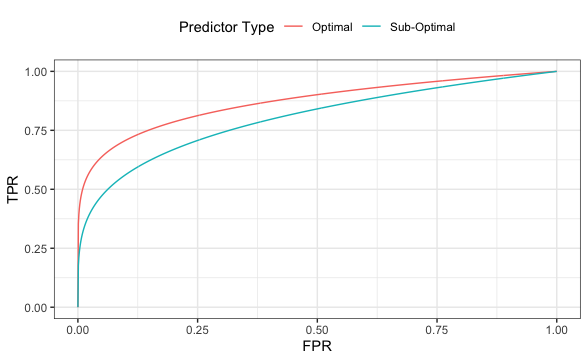
\includegraphics[scale=0.4]{roc_curves.png}
        \caption{ROC Curves.}
        \label{fig:roc_curves}
    \end{figure}
\end{frame}

\section{Optimal Extreme Event Prediction in Time Series Models}

\begin{frame}{The Pareto Distribution}
    For a random variable $X$ with CDF $F_X$, let $\bar{F}_X = 1 - F_X$.

    \smallskip
    
    $X$ has a Pareto distribution with shape parameter $\alpha > 0$ and scale parameter $x_m > 0$ if
    \[
    \bar{F}_X(x) = \left(\frac{x}{x_m}\right)^{-\alpha}
    \]
    for all $x \ge x_m$. Note that given $\lambda > 0$, for $x \ge \lambda x_m$,
    \[
    \P(\lambda X > x) = \bar{F}_X(x / \lambda) = \left(\frac{x}{\lambda x_m}\right)^{-\alpha}.
    \]
    The Pareto distribution is scale invariant.
\end{frame}

\begin{frame}{The Pareto Distribution}
    \begin{figure}[h!]
        \centering
        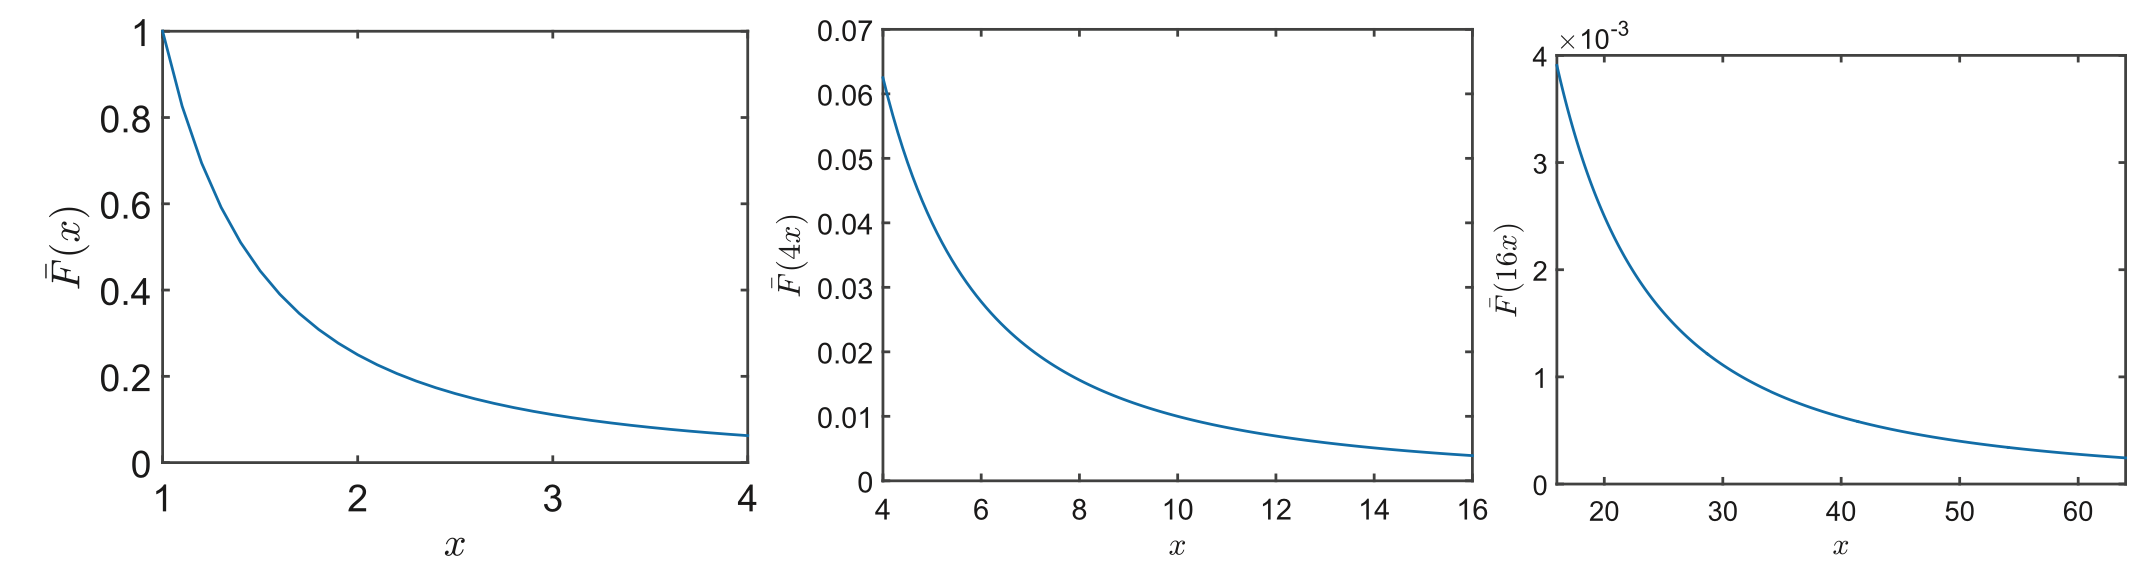
\includegraphics[scale=0.3]{scaled_paretos.png}
        \caption{A Pareto($\alpha = 2, x_m = 1$) distribution (left) and under rescalings (center, right) (from \cite{nair2022thef}).}
        \label{fig:scaled_paretos}
    \end{figure}
\end{frame}

\begin{frame}{Scale Invariance}
    \begin{definition}
        (The distribution of) $X$ is scale invariant if there exists $x_0 > 0$ and a continuous positive function $g$ such that
        \[
        \bar{F}_X(\lambda x) = g(\lambda)\bar{F}_X(x),
        \]
        for all $x, \lambda$ satisfying $x, \lambda x \ge x_0$.
    \end{definition}
    \begin{theorem}
        (The distribution of) $X$ is scale invariant if and only if $F_X$ has a power law tail, that is, there exists $x_0 > 0$, $c \ge 0$, and $\alpha > 0$ such that $\bar{F}_X(x) = c x^{-\alpha}$ for $x \ge x_0$.
    \end{theorem}
\end{frame}

\begin{frame}{Regularly and Slowly Varying Functions}
    For any function $g$ defined for all large $x$, if there exists $\alpha \in \R$ such that for all large $x$,
    \[
    \lim_{t \to \infty} \frac{g(t x)}{g(t)} = x^{-\alpha},
    \]
    then $g$ is called regularly varying with index $\alpha$ (written $g \in \RV_{\alpha}$). If $\alpha = 0$, then $g$ is called slowly varying.
    \begin{theorem}
        $g$ \in $\RV_{\alpha}$ if and only if there exists $\ell \in \RV_0$ such that for all large $x$,
        \[
        g(x) = x^{\alpha}\ell(x).
        \]
    \end{theorem}
\end{frame}

\begin{frame}{Asymptotic Scale Invariance}
    \begin{definition}
        (The distribution of) $X$ is asymptotically scale invariant if there exists a continuous positive function $g$ such that for any $\lambda > 0$,
        \[
        \lim_{x \to \infty} \frac{\bar{F}_X(\lambda x)}{\bar{F}_X(x)} = g(\lambda).
        \]
    \end{definition}
    \begin{theorem}
        (The distribution of) $X$ is asymptotically scale invariant if and only if it is regularly varying.
    \end{theorem}
\end{frame}

\begin{frame}{Regularly Varying Random Variables}
    \begin{definition}
        Let $X$ be a random variable defined on a probability space $(\Omega, F, P)$. $X$ is regularly varying with tail index $\alpha > 0$ if
        \begin{itemize}
            \item for all large $x$,
            \[
            \lim_{t \to \infty} \frac{\bar{F}_{|X|}(t x)}{\bar{F}_{|X|}(t)} = x^{-\alpha}.
            \]
            \item (tail balance condition) there exists $p_X \in [0, 1]$ such that
            \[
            \lim_{x \to \infty} \frac{\bar{F}_X(x)}{\bar{F}_{|X|}(x)} = p_X.
            \]
            $p_X$ is called the extremal skewness of (the distribution of) $X$.
        \end{itemize}
    \end{definition}
\end{frame}

\begin{frame}{Regularly Varying Random Variables}
    A simpler version we have been using:
    \begin{definition}
        A random variable $X$ is regularly varying (or heavy-tailed) with tail exponent $\alpha > 0$ if there exist $\sigma_{X, \pm} \ge 0$ such that
         % Unstar if you want to use the label
        \begin{equation*}\label{eq:tail_conds}
            P(X > x) \sim \sigma_{X, +}^{\alpha}x^{-\alpha} \text{ and } P(X < -x) \sim \sigma_{X, -}^{\alpha}x^{-\alpha}
        \end{equation*}
        as $x \to \infty$, where $\sigma_{X, +} + \sigma_{X, -} > 0$. The numbers $\sigma_{X, \pm}$ are called the right and left asymptotic scale coefficients, respectively.
    \end{definition}
\end{frame}

% \begin{frame}{Preliminaries on Regular Variation}
%     \begin{lemma}\label{lem:reg_var_properties}
%         Let $X$ and $Y$ be independent random variables that are regularly varying with tail exponent $\alpha$ and asymptotic scale coefficients $\sigma_{X, \pm}$ and $\sigma_{Y, \pm}$, respectively. Then
    
%         (i) For any $a \ne 0$, $a X$ is regularly varying with tail exponent $\alpha$ and asymptotic scale coefficients $|a|\sigma_{X, \pm{\rm sign}(a)}$.
        
%         (ii) $Z = X + Y$ is regularly varying with tail exponent $\alpha$ and asymptotic scale coefficients $\sigma_{Z, \pm}$, where $\sigma_{Z, \pm}^{\alpha} = \sigma_{X, \pm}^{\alpha} + \sigma_{Y, \pm}^{\alpha}$.
%     \end{lemma}
% \end{frame}

\begin{frame}{The Tail Dependence Coefficient}
    Recall that the level-$p_0$ tail dependence coefficient $\lambda_{p_0} = \lambda_{p_0}(Y, X)$ is defined by
    \[
    \lambda_{p_0} = P(Y > F_Y^{-1}(p_0) \mid X > F_X^{-1}(p_0))
    \]
    and the tail dependence coefficient $\lambda = \lambda(Y, X)$ is defined by
    \[
    \lambda = \lim_{p_0 \uparrow 1} \lambda_{p_0}
    \]
    if the limit exists.
\end{frame}

\begin{frame}{The Tail Dependence Coefficient}
    \begin{lemma}\label{lem:lambda_lem}
        Let $X$ and $\epsilon$ be independent random variables that are regularly varying with tail exponent $\alpha$ and asymptotic scale coefficients $\sigma_{X, \pm}$ and $\sigma_{\epsilon, \pm}$, respectively. For any $a \ne 0$, if $\sigma_{X, \sign(a)} > 0$, then
        \[
        \lambda(a X + \epsilon, X) = \frac{|a|^\alpha \sigma_{X, \sign(a)}^\alpha}{|a|^\alpha \sigma_{X, \sign(a)}^\alpha + \sigma_{\epsilon, +}^\alpha}.
        \]
    \end{lemma}
\end{frame}

\begin{frame}{Heavy-Tailed Time Series}
    Consider the model
    \begin{equation}\label{e:Y_t}
        Y_t  = \sum_{i=1}^{p} \phi_i Y_{t-i} + \epsilon_t,\ \ \ t\in \Z.
    \end{equation}
    Assume that
    \begin{itemize}
        \item the $\epsilon_t$'s are iid
        \item for all $t$, $\epsilon_t$ is independent of $Y_{t - 1}, Y_{t - 2}, \ldots$
    \end{itemize}

    \medskip

    Goal:
    \begin{center}
        Predict extreme events of the form $\{Y_{t + h} > F_Y^{-1}(p_0)\}$ using $\{Y_s, \ s \le t\}$    
    \end{center}
\end{frame}

\begin{frame}{Heavy-Tailed Time Series}
    Define $\Phi : \C \to \C$ by
    \[
    \Phi(z) = 1 - \sum_{i = 1}^p \phi_i z^i
    \]
    If $\Phi$'s roots lie outside the unit circle, then the model \eqref{e:Y_t} has a unique stationary solution:
    \begin{equation}\label{e:Y-as-a-moving-average}
        Y_t = \sum_{i = 0}^\infty a_i \epsilon_{t - i},
    \end{equation}
    where the $a_i$'s are given by
    \[
    \sum_{i = 0}^\infty a_i z^i = 1 / \Phi(z)
    \]
    when $|z| \le 1$.
\end{frame}

% \begin{frame}{Heavy-Tailed Time Series}
%     In the lemma below, $Y_t$ isn't necessarily given by \eqref{e:Y_t}, and the coefficients $a_i$ aren't necessarily those in the stationary solution \eqref{e:Y-as-a-moving-average}.
%     \begin{lemma}\label{lem:abs_as_conv}
%         Suppose that for all $t \in \Z$,
%         \begin{equation}\label{e:Y-as-a-moving-average2}
%             Y_t = \sum_{i = 0}^\infty a_i \epsilon_{t - i},
%         \end{equation}
%         where the $\epsilon_t$'s are iid. The series in \eqref{e:Y-as-a-moving-average2} converges absolutely and almost surely, provided that
%         \begin{equation}\label{e:convergence-sufficient-condition}
%         \P(|\epsilon_t| > x) \propto x^{-\alpha},\ \ \mbox{ and }\ \ \sum_{i = 0}^\infty |a_i|^{1 \wedge (\alpha - \delta)} <\infty 
%         \end{equation}
%         for some $\alpha > 0$ and $\delta \in (0, \alpha)$.
%     \end{lemma}
% \end{frame}

\begin{frame}{Heavy-Tailed Time Series}
    \begin{lemma}\label{lem:recursion}
        Define $\{\phi_{h, j}\}$ and $\{\psi_{h, j}\}$ as follows. When $-(p - 1) \le h \le 0$, for all $j$, set
        \[
        \phi_{h, j} = \delta_{|h|, j},\ \ \mbox{ and } \ \  \psi_{h, j} = 0,
        \]
        where $\delta$ is the Dirac delta.
    
        For all $h \ge 1$, define $\phi_{h, j}$ and $\psi_{h, j}$ recursively by
        \begin{align*}
            \phi_{h, j} &= \sum_{i = 1}^p \phi_i\phi_{h - i, j}, 0 \le j \le p - 1 \\
            \psi_{h, j} &=
            \begin{cases}
                \sum_{i = 1}^{(h - j) \wedge p} \phi_i\psi_{h - i, j}, & 1 \le j \le h - 1 \\
                1, & j = h
            \end{cases}
        \end{align*}
    \end{lemma}
\end{frame}

\begin{frame}{Heavy-Tailed Time Series}
    \begin{lemma}
        Then for all $h \ge -(p - 1)$,
        \begin{equation}\label{eq:y_t_plus_h_expr}
        Y_{t + h} = \sum_{j = 0}^{p - 1} \phi_{h, j}Y_{t - j} + \sum_{j = 1}^h \psi_{h, j}\epsilon_{t + j}. 
        \end{equation}
    \end{lemma}
\end{frame}

\begin{frame}{Heavy-Tailed Time Series}
    \begin{theorem}\label{thm:AR(p)-optimal-predictors}
    Let $\{Y_t\}$ be the unique stationary solution \eqref{e:Y-as-a-moving-average} of the model \eqref{e:Y_t}. For every $p_0 \in (0,1)$, the optimal predictor of $I(Y_{t+h}> F_Y^{-1}(p_0))$
    via $X:=(\begin{matrix}Y_t & \ldots & Y_{t - p + 1}\end{matrix})^{\top}$ is $I(k(X) > F_{k(X)}^{-1}(p_0))$, where 
    \[
    k(x) = \phi_h^{\top}x
    \]
    and
    \[
    \phi_h = (\begin{matrix}\phi_{h, 0} & \ldots & \phi_{h, p - 1}\end{matrix})^{\top}.
    \]
    \end{theorem}
\end{frame}

% \begin{frame}{Heavy-Tailed Time Series}
%     \begin{lemma}\label{lem:sigma_y_sum}
%         Let $\{\epsilon_i\}_{i = 0}^{\infty}$ be an iid sequence of random variables that are regularly varying with tail exponent $\alpha$ and let $\sigma_{\epsilon, \pm}$ be their common asymptotic scale coefficients. Let
%         \[
%         Y = \sum_{i = 0}^{\infty} a_i\epsilon_i.
%         \]
%         Assume that
%         \[
%         \sum_{i = 0}^{\infty} |a_i|^{\alpha / (\alpha + 1)} < \infty.
%         \]
%         Then $Y$ is regularly varying with tail exponent $\alpha$, and
%         \[
%         \sigma_{Y, +}^{\alpha} = \sum_{i = 0}^{\infty} |a_i|^{\alpha}\sigma_{\epsilon, \sign(a_i)}^{\alpha}.
%         \]
%     \end{lemma}
% \end{frame}

\begin{frame}{Heavy-Tailed Time Series}
    \begin{theorem}\label{thm:AR(p)-extreme-precision}
        Let $\{Y_t\}$ be the unique stationary solution \eqref{e:Y-as-a-moving-average} of the model \eqref{e:Y_t} and suppose that as $x \to \infty$
        \[
        \P(\pm \epsilon_t > x) \sim \sigma_{\epsilon, \pm}^\alpha x^{-\alpha}.
        \]
        
        Let $I(k(X) > F_{k(X)}^{-1}(p_0))$ be an optimal predictor of $I(Y_{t + h} > F_Y^{-1}(p_0))$. Then
        \[
        \lambda(h):= \lim_{p_0 \uparrow 1} \lambda_{p_0}(Y_{t+h}, k(X)) = 1 - \frac{\sigma_{\eta, +}^{\alpha}(h)}{\sigma_{Y, +}^{\alpha}(h)},
        \]
        where
        \[
        \sigma_{\eta, +}^{\alpha}(h) = \sum_{i = 1}^h |\psi_{h, i}|^{\alpha}\sigma_{\epsilon, \sign(\psi_{h, i})}^{\alpha} \text{ and } \sigma_{Y, +}^{\alpha}(h) = \sum_{i = 0}^{\infty} |a_i|^{\alpha}\sigma_{\epsilon, \sign(a_i)}^{\alpha}.
        \]
    \end{theorem}
\end{frame}

% \begin{frame}{Heavy-Tailed Time Series}
%     \begin{remark} It is technically difficult to obtain formulae for the precision $\lambda_{p_0}(h)$ for the
%     event $\{Y_{t+h} > F_Y^{-1}(p_0)\}$ for $p_0\in (0,1)$.  As shown in Theorem \ref{thm:AR(p)-extreme-precision}, however, using the theory of regular variation, one can establish the formula for the limiting {\em extremal optimal precision}. This asymptotic quantity $\lambda(h)$ quantifies the degree to which very extreme events can be predicted.
%     \end{remark}
% \end{frame}

% \begin{frame}{Heavy-Tailed Time Series}
%     \begin{remark}
%         Interestingly, if the innovations $\{\epsilon_t\}$ in \eqref{e:Y_t} are light-tailed, e.g., Gaussian, it can be shown that
%         $$
%         \lambda(h) = \lim_{p_0 \uparrow 1} \lambda_{p_0}(h) = 0.
%         $$
%         That is, the power in predicting very extreme events in Gaussian time series vanishes asymptotically.  In contrast, heavy-tailed
%         AR$(p)$ models, as seen from Theorem \ref{thm:AR(p)-extreme-precision} have asymptotically dependent extremes and therefore non-vanishing asymptotic optimal precision $\lambda(h)$.
%     \end{remark}
% \end{frame}

% \begin{frame}{Heavy-Tailed Time Series}
%     \begin{remark} \label{rem:Gaussian-vanishing-precision}
%         In \eqref{eq:y_t_plus_h_expr}, if the innovations are Gaussian, then the asymptotic optimal precision in predicting $Y_{t + h}$ via $Y_s$, $s \le t$, is zero. Indeed, this follows from the fact that if $\xi$ and $\eta$ are bivariate normal with correlation below 1, they are asymptotically independent, i.e., $\lambda(\xi, \eta) = 0$. For $p < 1$ though, Gaussian models may still provide some predictive power.
%     \end{remark}
% \end{frame}

\begin{frame}{State-Space Models for Heavy-Tailed Time Series with Covariates}
    Consider the linear state-space model
    \begin{equation}\label{eq:orig_ssm}
        \begin{split}
            X_t &= \sum_{j = 1}^q A_j X_{t - j} + \delta_t \\
            Y_t &= g \left( \sum_{j = 0}^{r - 1} \beta_j^{\top} X_{t - j} \right) + \epsilon_t,
        \end{split}
    \end{equation}
    where
    \begin{itemize}
        \item $X_t \in \R^d$ and the $\delta_t$'s are iid heavy-tailed
        \item $Y_t \in \R$, $g :\R \to \R$ is increasing, and the $\epsilon_t$'s are iid heavy--tailed with tail exponent $\alpha > 0$
        \item the $\delta_t$'s and the $\epsilon_t$'s are independent
    \end{itemize}
\end{frame}

\begin{frame}{State-Space Models for Heavy-Tailed Time Series with Covariates}
    Goal:
    \begin{center}
        Predict extreme events of the form $\{Y_{t + h} > F_Y^{-1}(p_0)\}$ using $\{X_s, \ s \le t\}$    
    \end{center}

    \medskip
    
    We may assume that $q = r$. Also, there exist $A \in \R^{dq \times dq}$ and $\beta \in \R^{dq}$ such that a solution to
    \begin{equation}\label{eq:new_ssm}
    \tilde X_t := A \tilde X_{t-1} + \tilde \delta_t\ \ \mbox{ and }\ \ Y_t = g(\beta^{\top}\tilde X_t) + \epsilon_t,
    \end{equation}
    where
    \[
    \tilde{X}_t := (X_t^{\top} \cdots X_{t - q + 1}^{\top})^{\top} \ \ \text{and} \ \
    \tilde{\delta}_t := (\begin{matrix} \delta_t^{\top} & 0 & \cdots & 0 \end{matrix})^{\top},
    \]
    is a solution to the original model \eqref{eq:orig_ssm}, so we may assume that $q = r = 1$.
\end{frame}

% \begin{frame}{State-Space Models for Heavy-Tailed Time Series with Covariates}
%     Set
%     \[
%     A :=
%     \left(\begin{array}{lllll}
%         A_1 & A_2 & \cdots & A_{q-1} & A_q\\
%         I_d & 0 & \cdots & 0 & 0 \\
%         0  & I_d & \cdots & 0& 0\\
%         \vdots & \vdots &  \ddots &\vdots & \vdots\\
%         0 & 0 & \cdots & I_d & 0
%     \end{array}\right) \ \ \mbox{ and } \ \
%     \beta := \left(\begin{array}{l}
%         \beta_1 \\ \beta_2 \\ \vdots \\ \beta_q
%     \end{array}\right) 
%     \]
% \end{frame}

\begin{frame}{State-Space Models for Heavy-Tailed Time Series with Covariates}
    Relation \eqref{eq:new_ssm} implies
    \begin{align*}
        Y_{t+h} &= g \Big( \beta^\top ( A \tilde X_{t+h-1} + \tilde  \delta_{t+h})\Big ) + \epsilon_{t+h} \\
        &= g \Big( \beta^\top A \tilde X_{t + h-1} +  \beta^\top \tilde  \delta_{t+h}  \Big) + \epsilon_{t+h} \\
        &\vdots \\
        &= g \Big( \beta^\top A^h \tilde X_t + \sum_{j=1}^h \beta^\top A^{h - j}\tilde  \delta_{t+j}  \Big) +  \epsilon_{t+h} \\
        &= g \Big( \beta^\top A^h \tilde X_t + \delta_{t,h} \Big) + \epsilon_{t+h},
    \end{align*}
    where 
    \begin{equation*}
    \delta_{t,h}:= \sum_{j=1}^h \beta^\top A^{h - j}\tilde  \delta_{t+j}.
    \end{equation*}
\end{frame}

\begin{frame}{State-Space Models for Heavy-Tailed Time Series with Covariates}
    \begin{proposition}
        Let $\{(\tilde X_t,Y_t)\}$ be a solution to the model \eqref{eq:new_ssm}. Assume that
        \begin{itemize}
            \item $\tilde{\delta}_s, \ s \ge t + 1$ and $\epsilon_s, \ s \ge t + 1$ are independent of $\tilde{X}_s, \ s \le t$
            \item $\tilde X_t$, $\delta_{t, h}$, and $\epsilon_{t+h}$ have densities
        \end{itemize}

        \medskip
        
        {\em (i)} The optimal predictor of $I(Y_{t+h}> F_{Y_{t+h}}^{-1}(p_0))$
        via $\{ \tilde X_s, s\le t\}$ takes the form $I(\beta^\top A^{h}\tilde X_t > \tau)$.
    \end{proposition}
\end{frame}

\begin{frame}{State-Space Models for Heavy-Tailed Time Series with Covariates}
    \begin{proposition}
        {\em (ii)} Suppose that the $\tilde{\delta}_t$'s are multivariate regularly varying with exponent $\nu>0$ and that the $\epsilon_t$'s are regularly varying with exponent
        $\alpha>0$ and scale coefficient $\sigma_{\epsilon,+}>0$.  Suppose moreover that $\{ (\tilde X_t, Y_t)\}$ is stationary, and
        that the function $g$ in the model \eqref{eq:new_ssm} is the identity. \\
        
        Then, the asymptotically optimal lag-$h$ precision is
        \begin{equation*}
        \lambda(Y_{t+h}, \beta^\top A^h \tilde X_t) = \left\{ \begin{array}{ll} 
        0 &, \mbox{ if } \nu>\alpha\\
        1- \sigma_{\delta_{t,h},+}^\nu / \sigma_{\beta^\top \tilde X_{0},+}^\nu &, \mbox{ if } \nu < \alpha\\
        1- (\sigma_{\delta_{t,h},+}^\nu + \sigma_{\epsilon,+}^\alpha) / \sigma_{Y,+}^\alpha &,\ \mbox{ if } \nu = \alpha,
        \end{array}\right.
        \end{equation*}
    \end{proposition}
\end{frame}    

% \begin{frame}{State-Space Models for Heavy-Tailed Time Series with Covariates}
%     \begin{remark}\label{rem:ss_phase_transition}
%         Observe that in the case when the measurement errors $\epsilon_k$ have strictly heavier tails 
%         than the innovations $\delta_k$ in the state-space equation, i.e., $\nu>\alpha$, it follows that the 
%         asymptotically optimal prediction precision is zero for all lags $h\ge 1$.  Indeed, in this  case, the measurement
%         noise simply dominates the state-space signal and there is vanishing information in the covariates $\{X_k\}$ about the extremes of $Y_k$.
%     \end{remark}
% \end{frame}

% \begin{frame}{State-Space Models for Heavy-Tailed Time Series with Covariates}
%     \begin{remark}\label{rem:ss_phase_transition_gauss}
%         If $\{(\tilde X_k, Y_k)\}$ is Gaussian and ${\rm Var}(\epsilon_{k+h})>0$ then the asymptotically
%         optimal precision  $\lambda(Y_{k+h}, \beta^\top A^h \tilde X_k) = 0$, for all $h\ge 1$. This follows, as in 
%         Remark \ref{rem:Gaussian-vanishing-precision}, from the fact that the jointly Gaussian random variables 
%         $Y_{k+h}$ and $\beta^\top A^h \tilde X_k$ have asymptotically independent extremes.
%     \end{remark}
% \end{frame}

\begin{frame}{A Simulation Study}
    Data was generated from the state-space model
    \begin{align*}
        X_t &= \sum_{j = 1}^5 0.5^j I_{16}X_{t - j} + \delta_t \\
        Y_t &= \sum_{j = 0}^4 0.5^j 1_{16}^{\top}X_{t - j} + \epsilon_t
    \end{align*}
    where
    \begin{itemize}
        \item $X_t \in \R^{16}$, $\delta_t \sim t_{\nu_{\delta}}(0, I_{16})$
        \item $Y_t \in \R$, $\epsilon_t \sim t_{\nu_{\epsilon}}$
        \item the $\delta_t$'s and $\epsilon_t$'s are mutually independent
    \end{itemize}
\end{frame}

\begin{frame}{A Simulation Study}
    Let 
    \[
    A =
    \left(
    \begin{matrix}
        0.5 \cdot I_{16} & 0.5^2 I_{16} & 0.5^3 I_{16} & 0.5^4 I_{16} & 0.5^5 I_{16} \\
        I_{16} & 0 & 0 & 0 & 0 \\
        0 & I_{16} & 0 & 0 & 0 \\
        0 & 0 & I_{16} & 0 & 0 \\
        0 & 0 & 0 & I_{16} & 0
    \end{matrix}
    \right), \
    \beta =
    \left(
    \begin{matrix}
        1_{16} \\
        0.5 \cdot 1_{16} \\
        0.5^2 1_{16} \\
        0.5^3 1_{16} \\
        0.5^4 1_{16}
    \end{matrix}
    \right)
    \]
    \[
    \tilde{X}_t = 
    \left(
    \begin{matrix}
        X_t^{\top} & X_{t - 1}^{\top} & X_{t - 2}^{\top} & X_{t - 3}^{\top} & X_{t - 4}^{\top}
    \end{matrix}
    \right)^{\top}
    \]
    The optimal predictor of $I(Y_{t + 1} > F_{Y_{t + 1}}^{-1}(p))$ is
    \[
    I(\beta^{\top} A\tilde{X}_t > \tau)
    \]
    for some $\tau$.
\end{frame}

\begin{frame}{A Simulation Study}
    Training and test sets were of the form
    \[
    \left(
    \begin{matrix}
    X_1^{\top} & \cdots & X_{-3}^{\top} & Y_2 \\
    \vdots & \ddots & \vdots & \vdots \\
    X_n^{\top} & \cdots & X_{n - 4}^{\top} & Y_{n + 1} \\
    \end{matrix}
    \right)
    =
    \left(
    \begin{matrix}
    \tilde{X}_1^{\top} & Y_2 \\
    \vdots & \vdots \\
    \tilde{X}_n^{\top} & Y_{n + 1} \\
    \end{matrix}
    \right).
    \]

    Given a new observation $\tilde{X}_*$, predict that $Y_*$ is extreme if $\beta^{\top} A\tilde{X}_*$ is above the $p$th sample quantile of $\{\beta^{\top} A\tilde{X}_1, \ldots, \beta^{\top} A\tilde{X}_n\}$.
\end{frame}

\begin{frame}{A Simulation Study}
    \begin{figure}[h!]
        \centering
        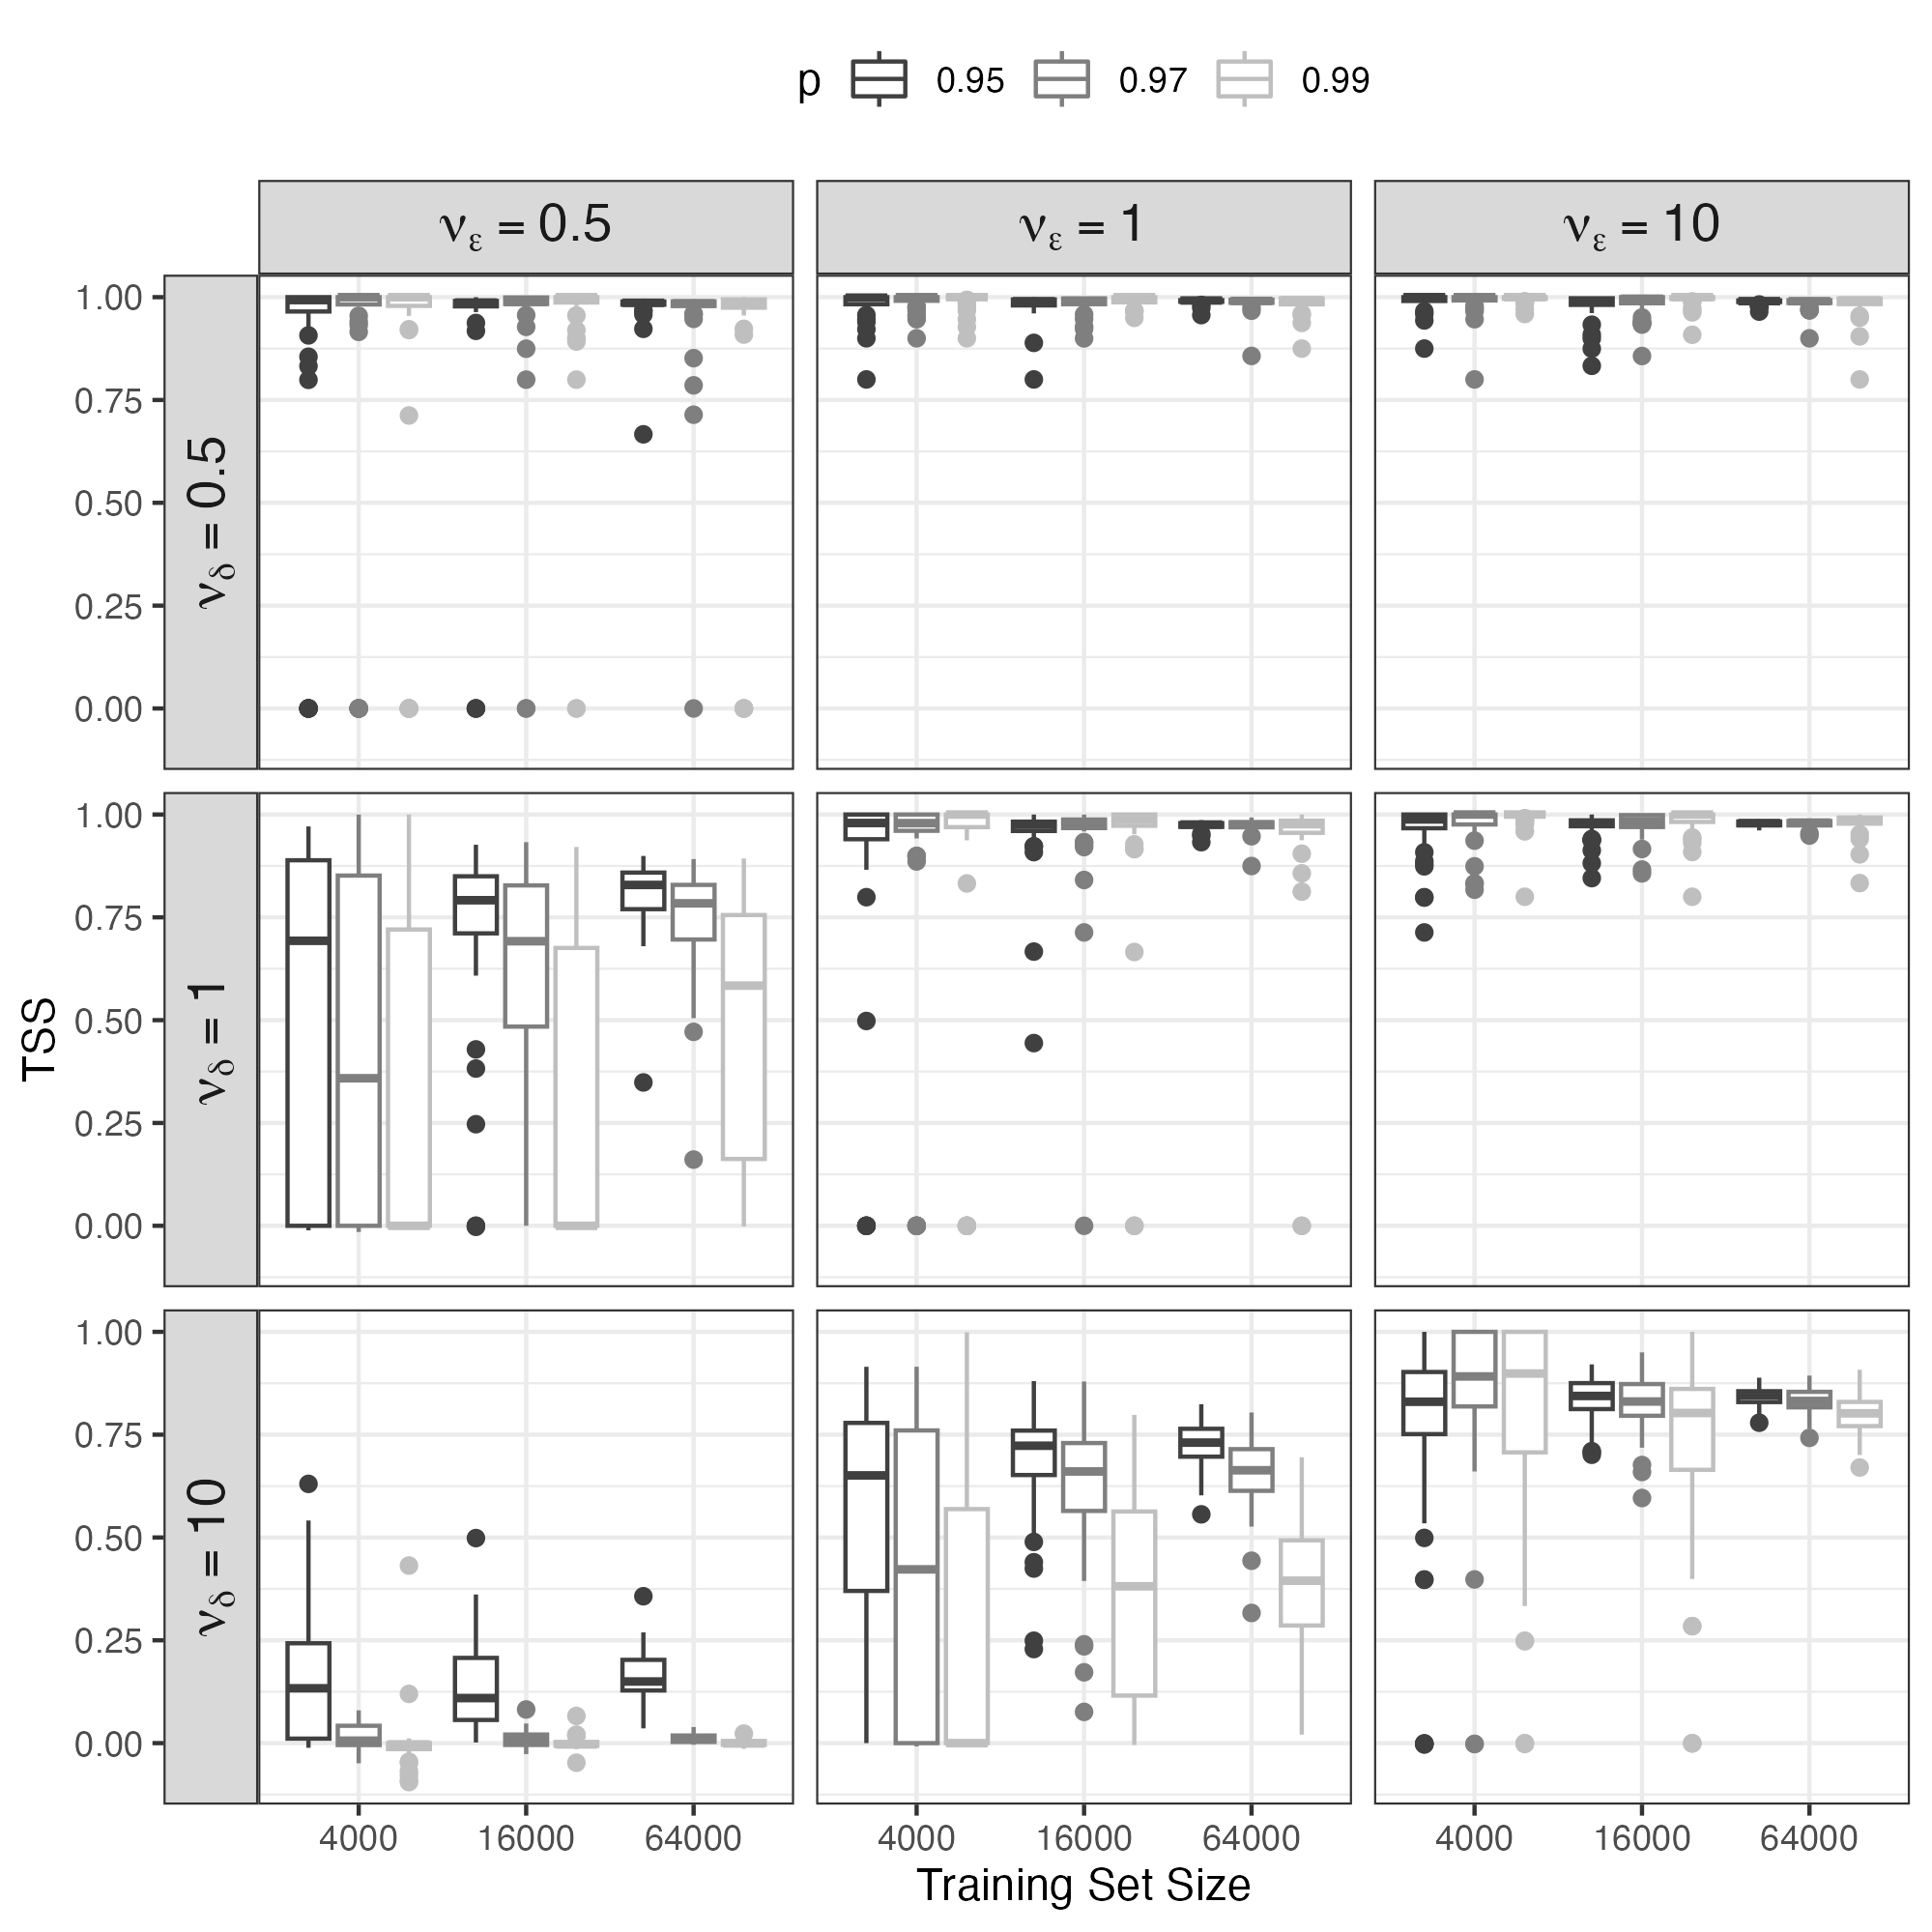
\includegraphics[scale=0.4]{sim_study07.png}
        \caption{Results of the simulation study.}
        \label{fig:sim_study07}
    \end{figure}
\end{frame}

\section{Data for Solar Flare Forecasting}

\begin{frame}{Data Information}
    \begin{itemize}
        \item Response (X-ray flux) data comes from the GOES satellites.
        % \begin{itemize}
        %     \item We use science-quality data, not operational data.
        %     \item The data is on a one-minute cadence.
        %     \item The data is mostly from solar cycle 24 (2008-2019), which saw unusually low levels of solar activity \cite{noaa2020hell}.
        % \end{itemize}
        \item Covariate (SHARP parameter) data comes from the Solar Dynamics Observatory (SDO).
        % \begin{itemize}
        %     \item Raw covariates are SHARP parameters, variables that describe flare-producing active regions in various ways \cite{bobra2014theh}.
        %     \item The data is on a 12-minute cadence.
        % \end{itemize}
    \end{itemize}

    The response and covariate data was combined as follows:
    \begin{itemize}
        \item Impute missing flux and SHARP parameter values
        % by taking the maximum across active regions at each time
        \item Aggregate SHARP parameter data across HARPs 
        \item Join aggregated SHARP time series to flux time series
    \end{itemize}
    The final time series consists of $\num[group-separator={,}]{287635}$ observations.
\end{frame}

\begin{frame}{Nonstationarity}
    \begin{figure}
        \centering
        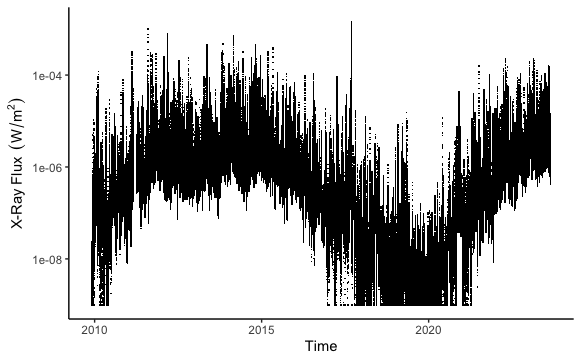
\includegraphics[scale=0.5]{flux_plot.png}
        \caption{The GOES X-ray flux time series.}
        \label{fig:flux_plot}
    \end{figure}
\end{frame}

\begin{frame}{Missing and Low Quality Values}
    \begin{figure}
        \centering
        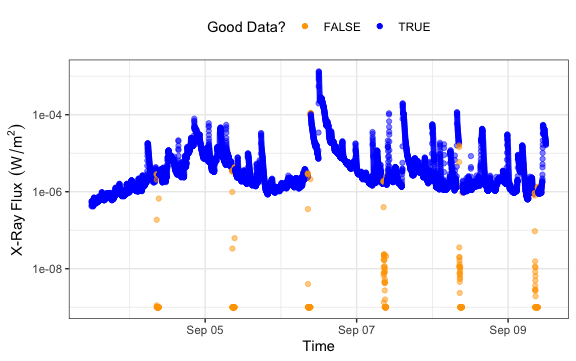
\includegraphics[scale=0.5]{flux_20170906.png}
        \caption{The X-Ray flux, 9/3/17-9/9/17.}
        \label{fig:flux_20170906}
    \end{figure}
\end{frame}

\begin{frame}{Missing and Low Quality Values}
    \begin{figure}[!htb]
        \centering
        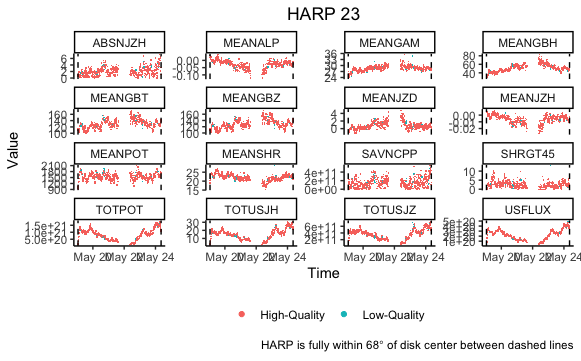
\includegraphics[scale=0.5]{harp23.png}
        \caption{SHARP parameter time series for HARP 23.}
        \label{fig:na_props_flux}
    \end{figure}
\end{frame}

\begin{frame}{Missing and Low Quality Values}
    \begin{figure}[!htb]
        \centering
        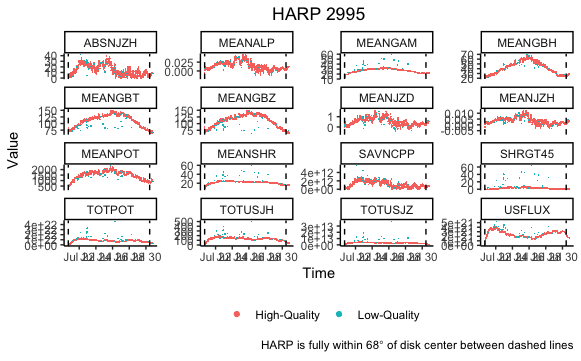
\includegraphics[scale=0.5]{harp2995.png}
        \caption{SHARP parameter time series for HARP 2995.}
        \label{fig:na_props_flux}
    \end{figure}
\end{frame}

% \begin{frame}{Missing and Low Quality Values}
%     \begin{figure}[!htb]
%         \centering
%         \includegraphics[scale=0.25]{na_props_flux.png}
%         \caption{Monthly proportions of times with no or a bad flux.}
%         \label{fig:na_props_flux}
%     \end{figure}
% \end{frame}

% \begin{frame}{Missing and Low Quality Values}
%     \begin{figure}[!htb]
%         \centering
%         \includegraphics[scale=0.25]{na_props_sharp.png}
%         \caption{Monthly proportions of times with no SHARP parameters.}
%         \label{fig:na_props_sharp}
%     \end{figure}
% \end{frame}

\begin{frame}{High Dimensionality}
    \begin{figure}[!htb]
        \centering
        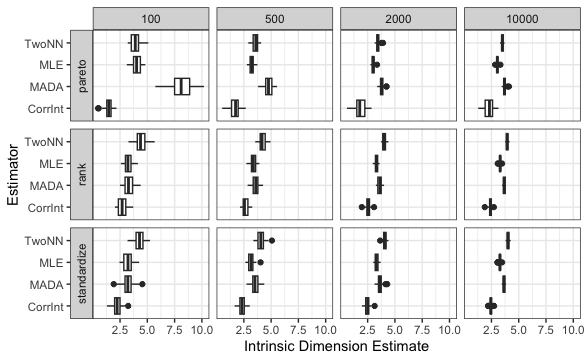
\includegraphics[scale=0.5]{intrinsic_dim_ests.png}
        \caption{Estimates of the intrinsic dimension of the SHARP parameters.}
        \label{fig:intrinsic_dim_ests}
    \end{figure}
\end{frame}

\begin{frame}{Heavy Tails}
    \begin{figure}[h!]
        \centering
        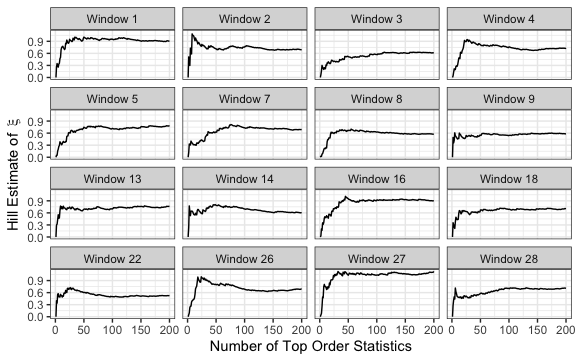
\includegraphics[scale=0.4]{hill_ests.png}
        \caption{Hill estimates of $\xi$ computed over consecutive $\num[group-separator={,}]{10000}$-observation windows of the flux time series. The windows included in this plot were randomly selected.}
        \label{fig:hill_ests}
    \end{figure}
\end{frame}

\begin{frame}{Heavy Tails}
    \begin{figure}
        \centering
        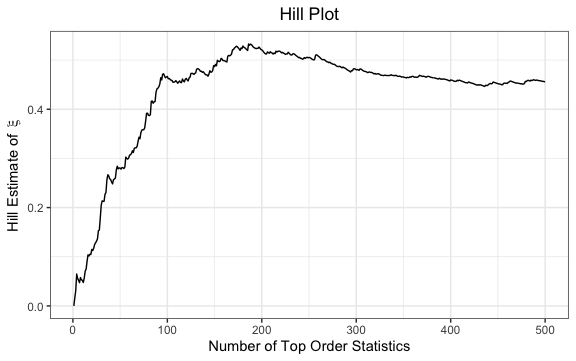
\includegraphics[scale=0.5]{hill_plot.png}
        \caption{One particular Hill plot for the X-Ray flux.}
        \label{fig:hill_plot}
    \end{figure}
\end{frame}

% \begin{frame}{X-Ray Flux Data}
%     \begin{figure}
%         \centering
%         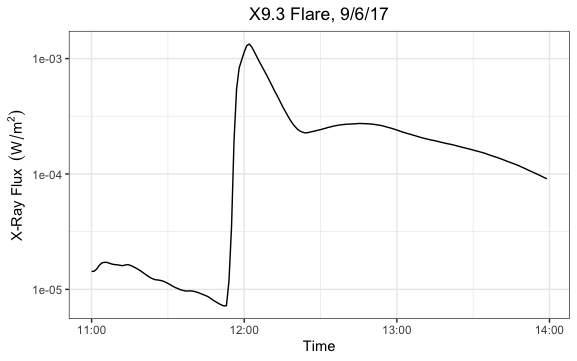
\includegraphics[scale=0.5]{flare_flux_example.png}
%         \caption{The X-ray flux for an X-class flare}
%         \label{fig:flare_flux_example}
%     \end{figure}
% \end{frame}

\section{A Statistical Framework for Solar Flare Forecasting}
\label{sect:forecast_framework}

\begin{frame}{Preprocessing Approaches}
    Marginal transformations:
    \begin{itemize}
        \item Standardization
        \begin{itemize}
            \item $X_{i j} \rightarrow (X_{i j} - \bar{X}_j) / s_j$
        \end{itemize}
        \item Let $\hat{F}_j$ be the empirical CDF of SHARP parameter $j$.
        \item Rank transformation
        \begin{itemize}
            \item $X_{i j} \rightarrow \hat{F}_j(X_{i j})$
        \end{itemize}
        \item Pareto transformation
        \begin{itemize}
            \item $X_{i j} \rightarrow \frac{1}{1 - \hat{F}_j(X_{i j})}$
        \end{itemize}
    \end{itemize}
\end{frame}

\begin{frame}{Preprocessing Approaches}
    Nonlinear dimensionality reduction:
    \begin{itemize}
        \item One technique is locally linear embedding (LLE) \cite{roweis2000nonl}.
        \item LLE assumes that observations $X_1, \ldots, X_n \in \R^D$ lie on/near a manifold of dimension $d \ll D$.
        \item LLE steps:
        \begin{enumerate}
            \item Find the $K$ NNs of each $X_i$.
            \item For each $X_i$, calculate weights $w_{i j}$ for reconstructing $X_i$ from its neighbors as $\sum_j w_{i j}X_j$.
            \item Compute $Y_1, \ldots, Y_n \in \R^d$ to minimize $\sum_{i = 1}^n \|Y_i - \sum_j w_{i j}Y_j\|_2^2$.
        \end{enumerate}
        \item $Y_1, \ldots, Y_n$ are the embeddings of $X_1, \ldots, X_n$, respectively, in the manifold.
        \item We apply LLE to construct four composite features from the SHARP parameters.
    \end{itemize}
\end{frame}

\begin{frame}{Preprocessing Approaches}
    Spline transformation of covariates:
    \begin{itemize}
        \item A linear combination of the covariates has the form
        \[
        X^{\top}\beta = \sum_{i = 1}^d \beta_i X_i.
        \]
        \item To increase flexibility, we replace $\beta_i X_i$ with $s_i(X_i)$, where $s_i$ is a natural spline.
        \item Sample quantiles of $X_i$ are used as knots.
    \end{itemize}
\end{frame}

\begin{frame}{Forecasting via Empirical Tail Dependence Maximization}
    Given training data $(X_1, Y_1), \ldots, (X_n, Y_n)$, the level-$p_0$ empirical tail dependence coefficient is
    \[
    \hat{\lambda}_{p_0}(Y, g(X)) = \frac{1}{n(1 - p_0)}\sum_{i = 1}^n I(g(X_i) \ge \hat{F}_{g(X)}^{-1}(p_0))I(Y_i \ge \hat{F}_{Y}^{-1}(p_0)),
    \]
    We compute
    \[
    \hat{g} = \argmin_{g \in \mathcal{C}} \left[-\hat{\lambda}_{p_0}(Y, g(X)) + \text{penalty}(g)\right].
    \]
\end{frame}

\begin{frame}{Forecasting via Empirical Tail Dependence Maximization}
    A natural class of predictors:
    \[
    \mathcal{C} = \{g : g(x) = x^{\top}\beta, \beta \in S^{d - 1}\}.
    \]
    We compute
    \[
    \hat{\beta} = \argmin_{\beta \in S^{d - 1}} \left[-\hat{\lambda}_{p_0}(Y, X^{\top}\beta) + \lambda\|\beta - \hat{\beta}_{\text{prev}}\|_2\right].
    \]
    Set $\hat{g}(x) = x^{\top}\hat{\beta}$. Prediction steps:
    \begin{itemize}
        \item Calculate the $p$th sample quantile $\hat{F}_{\hat{g}(X)}^{-1}(p_0)$ of $\hat{g}(X_1), \ldots, \hat{g}(X_n)$.
        \item Given a new observation $X_*$, predict that $Y_* > F_{Y}^{-1}(p_0)$ if $\hat{g}(X_*) > \hat{F}_{\hat{g}(X)}^{-1}(p_0)$.
    \end{itemize}
\end{frame}

\begin{frame}{Results}
    \begin{figure}[!htb]
        \centering
        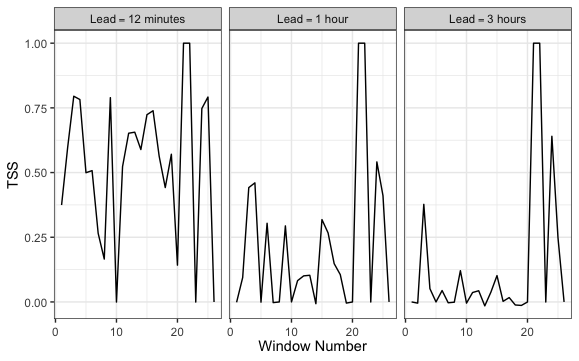
\includegraphics[scale=0.5]{0601_results.png}
        \caption{Results for LLE-constructed covariates.}
        \label{fig:0601_results}
    \end{figure}
\end{frame}

\begin{frame}{Results}
    \begin{figure}[!htb]
        \centering
        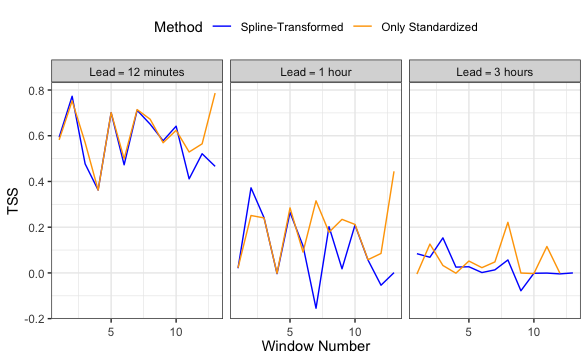
\includegraphics[scale=0.5]{0101_results.png}
        \caption{More results, for hand-picked covariates.}
        \label{fig:0101_results}
    \end{figure}
\end{frame}

\begin{frame}{Results}
    \begin{figure}[!htb]
        \centering
        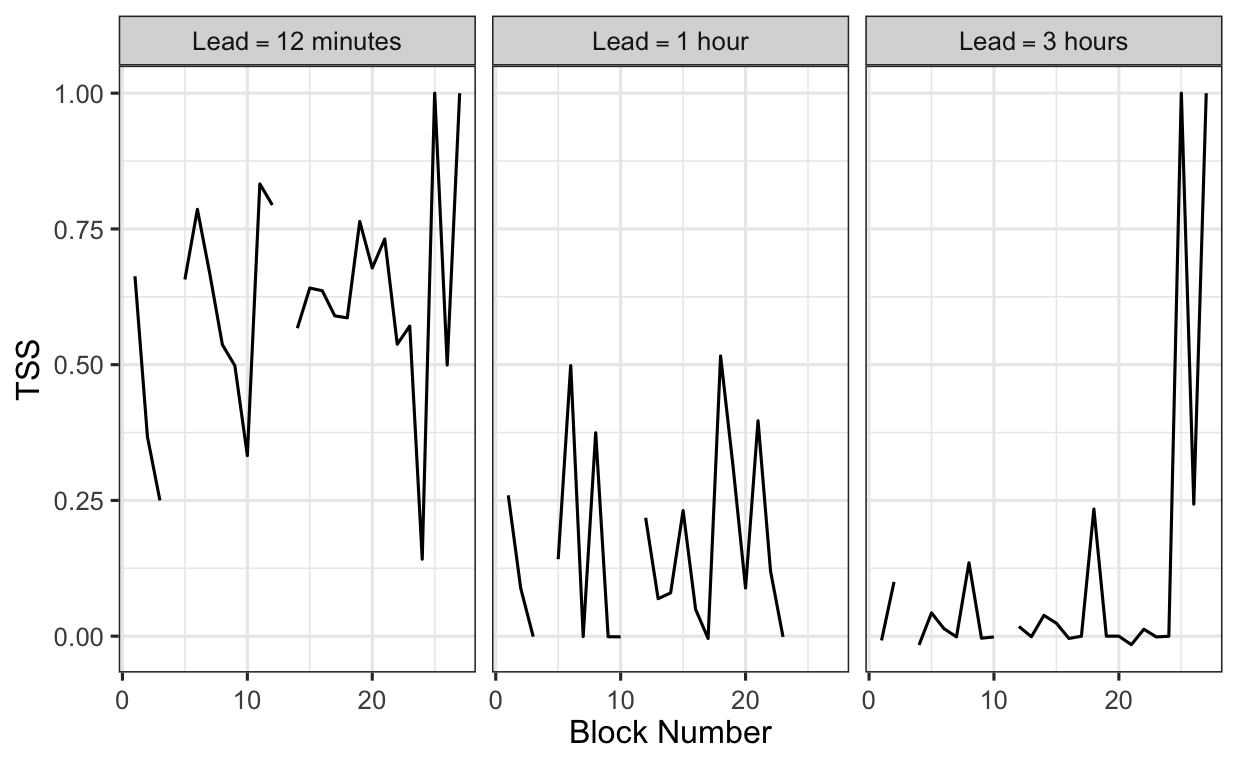
\includegraphics[scale=0.25]{0901_results.png}
        \caption{More results, for hand-picked covariates and imputed data.}
        \label{fig:0901_results}
    \end{figure}
\end{frame}

\begin{frame}{Results}
    \begin{figure}[!htb]
        \centering
        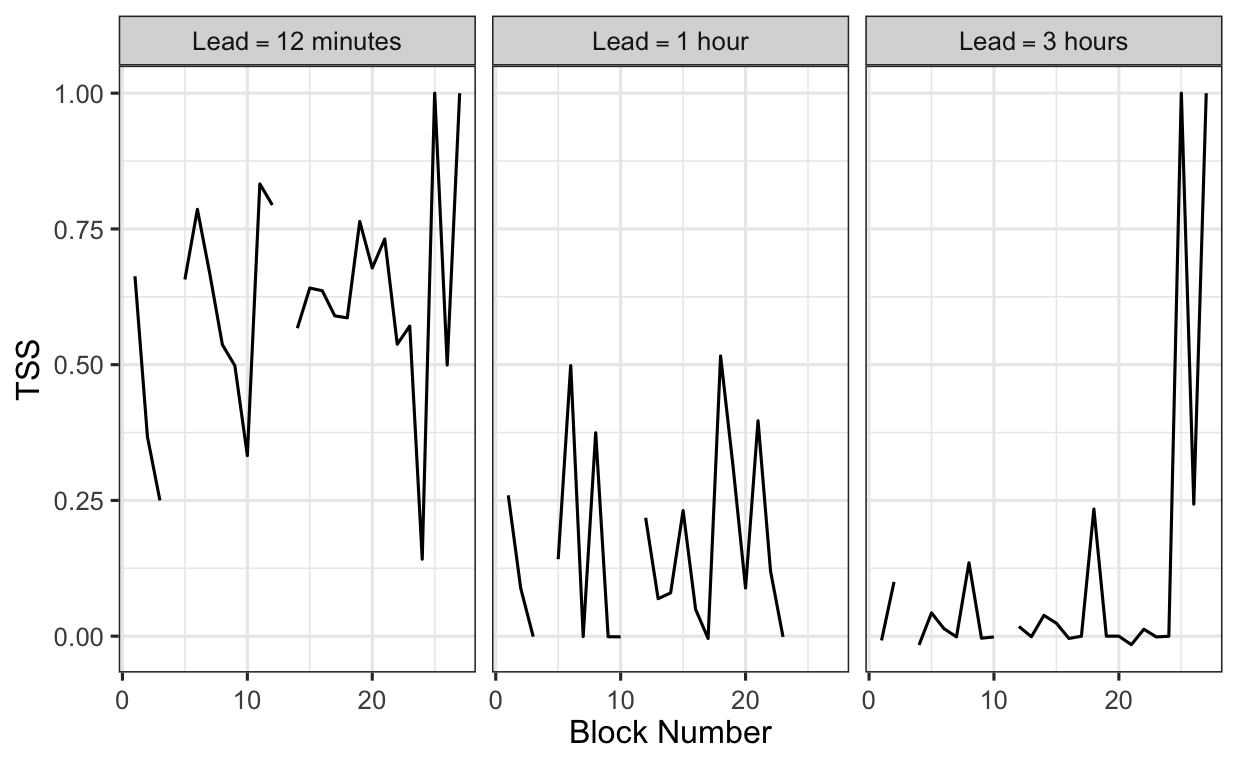
\includegraphics[scale=0.25]{0901_results.png}
        \caption{More results, for hand-picked covariates and imputed data.}
        \label{fig:0901_results}
    \end{figure}
\end{frame}

% \begin{frame}{Future Work}
%     \begin{itemize}
%         \item Tail dependence approach: consider functions $g(X)$ that are copulas or neural networks
%         \item Logistic regression
%         \item State space models
%     \end{itemize}
% \end{frame}

% \begin{frame}{Preprocessing}
%     \begin{figure}
%         \centering
%         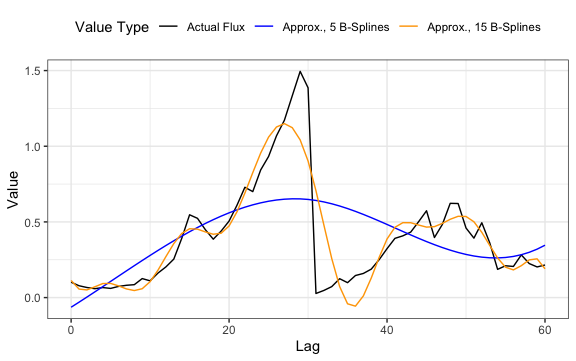
\includegraphics[scale=0.5]{spline_plots.png}
%         \caption{A sequence of flux values and its B-spline basis approximations.}
%         \label{fig:spline_plots}
%     \end{figure}
% \end{frame}

\begin{frame}[allowframebreaks]{References}
    \nocite{*}
    \printbibliography
\end{frame}

\section{Appendix}

\begin{frame}{SHARP Parameter Data}
    \begin{figure}
        \centering
        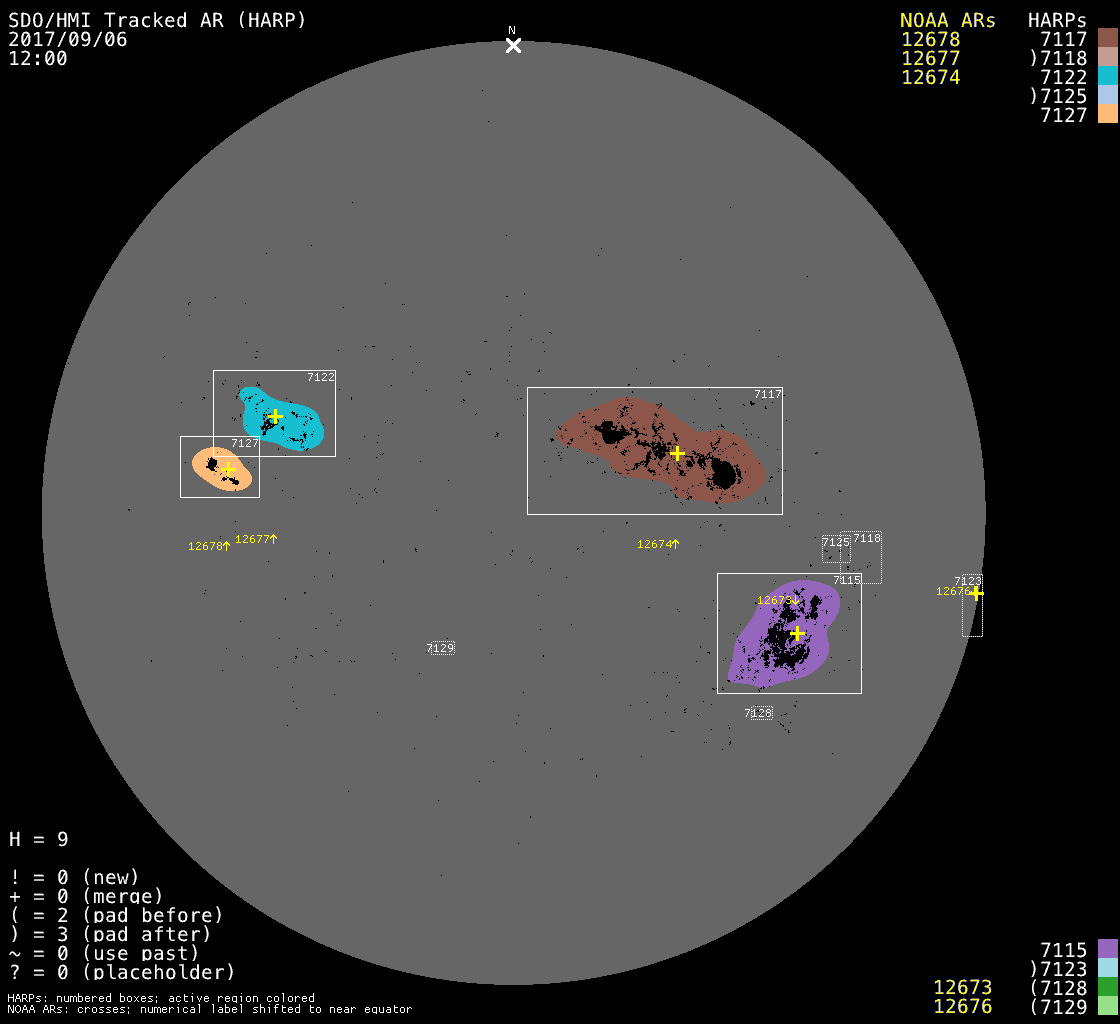
\includegraphics[scale=0.19]{magnetogram_20170906.png}
        \caption{HARPs on 9/6/17.}
        \label{fig:magnetogram_20170906}
    \end{figure}
\end{frame}

\begin{frame}{SHARP Parameter Data}
    \begin{figure}
        \centering
        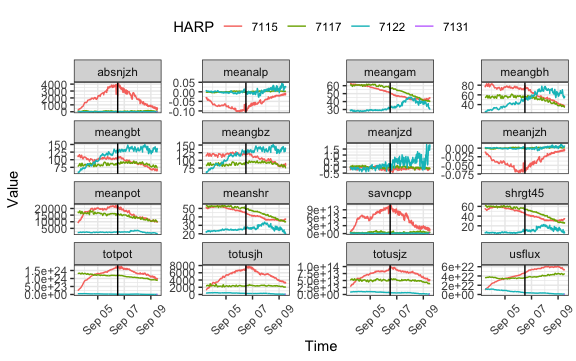
\includegraphics[scale=0.55]{sharp_params_20170906.png}
        \caption{SHARP parameters, 9/3/17-9/9/17}
        \label{fig:sharp_params_20170906}
    \end{figure}
\end{frame}

\end{document}